\documentclass[conference]{IEEEtran}
\usepackage{cite}
\usepackage{amsmath,amssymb,amsfonts}
\usepackage{algorithmic}
\usepackage{graphicx}
\usepackage{textcomp}
\usepackage{enumitem}
\usepackage{balance}
\usepackage{hyperref}
\bibliographystyle{IEEETran}

\begin{document}

\title{Automatic Completion of Missing Spreadsheet Data using Machine Learning Techniques}

\author{\IEEEauthorblockN{Noah Kruiper, Tyson Moore}
\IEEEauthorblockA{\textit{School of Electrical Engineering \& Computer Science} \\
\textit{University of Ottawa}\\
Ottawa, Canada \\
\{nkrui088, tmoor092\}@uottawa.ca}
}

\maketitle

\begin{abstract}
In spreadsheet software, auto-fill is traditionally used to continue simple sequences or patterns. It cannot generally fill missing data from complex datasets. This paper discusses a method of extending this auto-fill functionality to use machine learning models, trained entirely on the same dataset into which it will be inserting missing values. Each machine learning model is independently evaluated, and the most accurate is chosen on a per-data-type basis. The results show acceptable performance on simple datasets, and list potential improvements for future iterations of the software.
\end{abstract}

\begin{IEEEkeywords}
machine learning, spreadsheets, autocompletion
\end{IEEEkeywords}

\section{Introduction}
Computer spreadsheet programs have generally limited auto-fill functionality. It may only work on sequences of numbers or dates, it may be unable to interpolate gaps in data, and it may be limited to certain rules defined by the spreadsheet vendor. Adobe's \textit{Content-Aware Fill} feature\footnote{\url{https://helpx.adobe.com/photoshop/using/content-aware-fill.html}} in its Photoshop graphics editing software has the effect of filling in unknown properties of images; for example, restoring a background after removing an unwanted subject from the foreground.

To this end, we have designed SheetComplete: an application designed to emulate this content-aware fill functionality on spreadsheets. To accomplish this goal, SheetComplete evaluates multiple machine learning algorithms for each dataset, filling in gaps with the algorithm's predictions. This paper discusses related research in the intersection of spreadsheets and machine learning, SheetComplete's design process, implementation details, testing results, and potential future improvements and further research.

\section{Related Work}
Several authors and organizations have researched using machine learning with spreadsheet data, and running multiple machine learning algorithms against a single dataset to determine the best performing classifier/regressor.

Microsoft -- creator of the popular Excel spreadsheet application -- filed for a U.S. patent entitled \textit{Predicting spreadsheet properties} \cite{singh_predicting_2018}. The patent application details a method of using abstract spreadsheet representations as input to machine learning prediction functions, where the machine learning algorithms are trained on ``a plurality of previously-created spreadsheets.'' An example in the patent is discovering errors in complete datasets.

Although the patent is similar to SheetComplete, the functionality differs significantly between the two applications. Essentially, the Excel machine learning functionality recognizes patterns in existing data, and uses a curated data source API (Bing Knowledge Graph) to retrieve further information relating to that data. For example, population data for a list of towns, or companies' financial performance data given a list of stock indexes \cite{lardinois_excel_2018}.

There are many previous works that employ training multiple machine learning algorithms and assessing their performance. For example, \cite{kim_classification_2017} discusses training several algorithms against a \textit{dummy classifier} to identify the best-performing machine learning classifier for a static dataset of human-categorized tweets. More specifically, \cite{russo_comparing_2018} used normalized scores of multiple machine learning algorithms for a pharmaceutical application, but again used a static dataset.

The approaches chosen by these authors worked for their specific purposes. However, SheetComplete's application is more general than those identified above. Unlike the preceding examples, SheetComplete works with arbitrary datasets, as it performs training and assessment activities uniquely for each input spreadsheet. Moreover, it performs a granular assessment of machine learning algorithms for each input data \textit{field}, rather than relying on a single best-performing regressor for the entire dataset. These characteristics will be outline in detail in the following section.

\section{Methodology}
We developed the following general algorithm to guide our implementation. Fig.~\ref{flow} shows a general representation of data flow through SheetComplete.

\begin{figure}[htbp]
\centerline{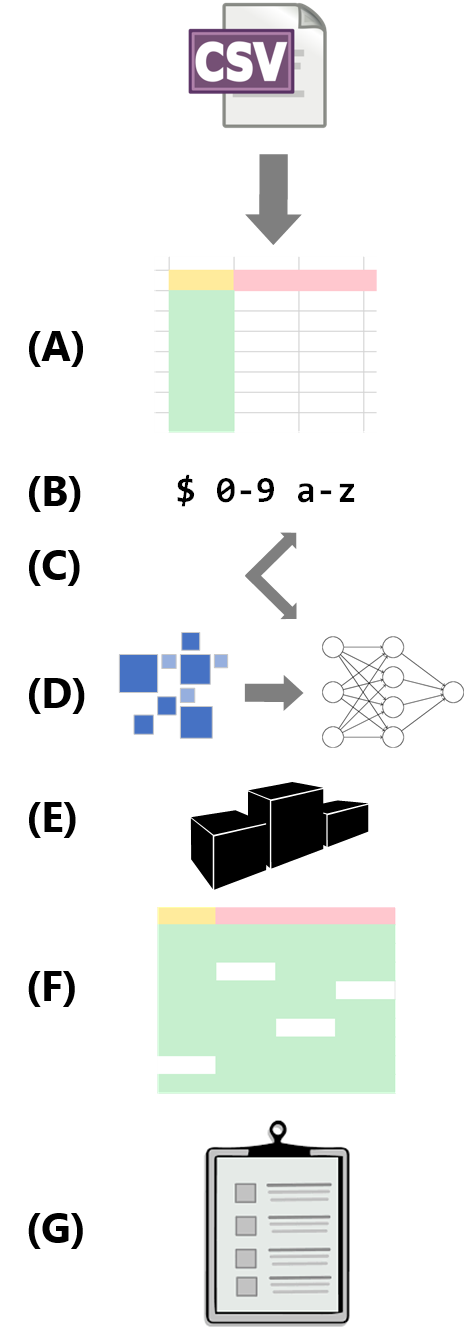
\includegraphics[height=0.5\textheight]{img/flow.png}}
\caption{Flow of data through SheetComplete application.}
\label{flow}
\end{figure}

\subsection{Determine Dataset Directionality}
First, the orientation of the data must be determined. Spreadsheets will have data series running left-to-right (in a single row) or top-to-bottom (in a single column). We need to determine where the datasets are located in the document, extract them, and determine whether or not they have headers.

At present, SheetComplete can only process CSV files with headers, but can work with spreadsheets in either column orientation or row orientation. If the provided spreadsheet has its records oriented row-wise, it is transposed internally to be processed as column-wise (and then transposed back upon completion to be the same orientation as the input). The application cannot currently handle complex spreadsheets; for example, those with multiple datasets in a single column, or with varying data directionality.

\subsection{Determine Dataset Type}
We must determine what data type is expected for each column. As the SheetComplete system is only capable of filling in numerical data, we must focus exclusively on columns with numbers which can be processed by the machine learning regressors. 

\subsection{Sort and Classify Datasets}
The machine learning regressors must be trained and assessed based only on complete records. We must therefore divide the datasets twice: first into complete and incomplete records, and then into training and assessment sets. By default, SheetComplete uses an 80/20 train/test split.

This step also identifies which of the data types have incomplete records to avoid wasted computation time (i.e. it is unnecessary to evaluate algorithms for a complete dataset, since no predictions are needed).

\subsection{Train Networks}
For each column with missing data, we train a network with each candidate algorithm using the training records set. We then have multiple potential prediction models for each column with missing records.

\subsection{Assess Networks}
In order to make predictions and fill in missing data, we must compare the prediction results between allt he models trained in the previous step to determine an optimal regressor for each column. The process for this step is as follows:
\begin{enumerate}[label=(\alph*)]
\item Remove one column of data (using the subset of columns with missing data) from the entire test set \label{a}
\item Use each network trained for that column to complete the missing dataset \label{b}
\item Compare the output from \ref{b} to the complete assessment set (i.e. the expected result) \label{c}
\item Repeat steps \ref{a}-\ref{c} for each dataset in the spreadsheet
\item For each dataset, determine which network produces the most appropriate result based on \ref{c}
\end{enumerate}

Functionally, this is implemented using the $R^2$ score for each regressor. A value of $1$ represents a perfect regression, while lower values represent poorer fits.\footnote{Unlike traditional $R^2$ scores, the algorithms can generate scores that are arbitrarily negative. These scores were seen with the Multi-Layer Perceptron (MLP) for certain types of data.}

\subsection{Populate Missing Data}
Using the best network for each data type, populate the missing cells from the incomplete records set.

\subsection{Produce a Report}
Generate a summary of the network used for each data type, the data that was filled in, and the efficacy of the network as determined in previous steps.

\section{Setup}
Our setup for SheetComplete is similar to many machine learning processes taught to beginners, using Python packages. The following sections describe implementation choices in detail, based on requirements and our algorithm.

\subsection{Environment}
To develop SheetComplete, we used Python~3.7.1 on \mbox{macOS} and Windows with the libraries \texttt{scikit-learn} and \texttt{pandas} for machine learning and data manipulation respectively. The \texttt{scikit-learn} library came highly recommended by the project sponsor, with many useful features for machine learning beginners like ourselves. These libraries seem to be the most frequently-used in academic scenarios, as they are plug-and-play libraries (i.e. one does not need to be a data scientist to adjust parameters of the classifiers/regressors). As we are both new to Python, \texttt{pandas} was new to us, but is nonetheless a core library with provides important data structures, useful with machine learning. 

\subsection{Algorithm Details}
To determine the directionality of the dataset, we used the internal \texttt{csv} functions within Python, along with \texttt{pandas} to figure out in which direction the header is oriented. After the data has been loaded into a \texttt{pandas} \textit{dataframe} (an array-like structure), the data type of each column can be determined using the \texttt{.dtypes} property. \texttt{pandas} was also useful to split the data based on the completeness of rows, as dataframes have the \texttt{.dropna()} function which eliminates incomplete records, and \texttt{.isna().any()} which identifies columns with any missing cells.

\subsection{Testing}
For testing, we used a variety of different spreadsheets. For each example, we removed the data from a random selection of cells, and processed the CSV with SheetComplete. Afterwards, we compared the predicted values to the removed data, and compared the accuracy of the predicted data to the scores assigned to each algorithm within SheetComplete (provided by the program's reported output).

An example illustrated below uses the first 10,000 lines of an open data set \cite{government_of_canada_economics_2018} from the Government of Canada. In Fig.~\ref{gc-1}, one can see a trivial example where the selected algorithm has discovered consistent numerical data, and fills it in appropriately.

\begin{figure}[htbp]
\centerline{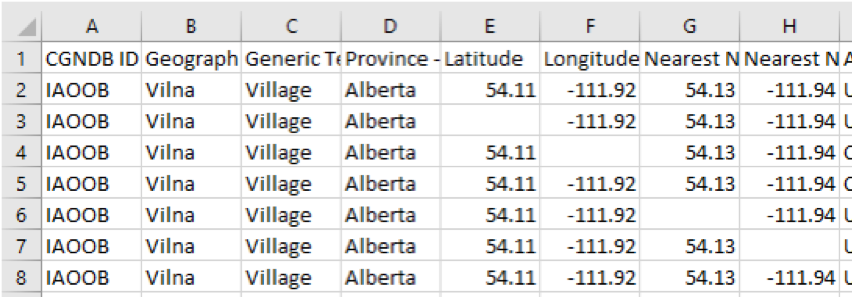
\includegraphics[width=\columnwidth]{img/gc-empty1.png}}
\vspace{2mm}
\centerline{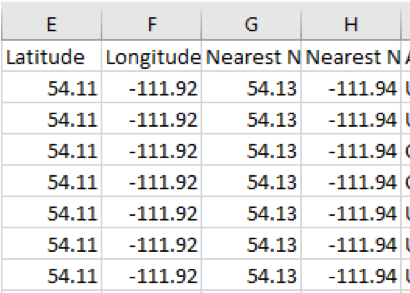
\includegraphics[scale=0.7]{img/gc-filled1.png}}
\caption{Trivial autofill application -- empty cells (top) and filled with SheetComplete (bottom).}
\label{gc-1}
\end{figure}

We also see that if the input dataset is sufficiently large, the machine learning algorithms generate data that is within the realm of possibility -- sometimes very close. Fig.~\ref{gc-2} shows an example of this from the same sheet. The autofilled value -- based solely on other pre-existing values in the same sheet -- is within $0.06\%$ of the original value.

\begin{figure}[htbp]
\centerline{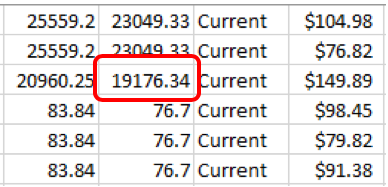
\includegraphics[width=0.7\columnwidth]{img/gc-start2.png}}
\vspace{3mm}
\centerline{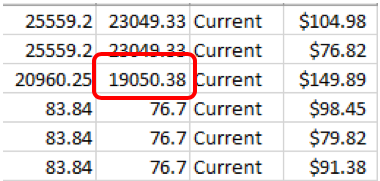
\includegraphics[width=0.7\columnwidth]{img/gc-filled2.png}}
\caption{More complicated application -- original data (top), and the new data filled with SheetComplete (bottom).}
\label{gc-2}
\end{figure}

Where the patterns/correlations are non-obvious -- or where the records are not predominantly numerical -- the generated results seem to be within the valid range for the dataset, though are significantly further off from the expected value. Fig.~\ref{gc-3} illustrates an example of this case. Although the resulting value is neither the minimum or maximum in its column, it is still more than $65\%$ off from its expected value. As with any machine learning problem, the accuracy of the predictions will improve with the size of the training set, and with data that can be mathematically modelled (even if that mathematical model is very complex).

\begin{figure}[htbp]
\centerline{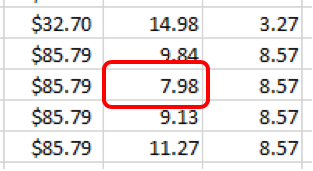
\includegraphics[width=0.5\columnwidth]{img/gc-start3.png}}
\vspace{2mm}
\centerline{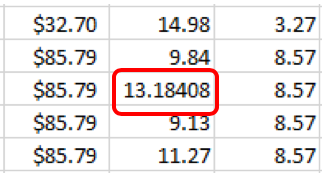
\includegraphics[width=0.5\columnwidth]{img/gc-filled3.png}}
\caption{An example of SheetComplete producing plausible -- but incorrect -- values. Starting value (top), and filled value with SheetComplete (bottom).}
\label{gc-3}
\end{figure}

Finally, Fig.~\ref{accuracy} shows a sample report from SheetComplete, showing the $R^2$ scores for the implemented regressors on a particular column of the test data. One can see that -- since the data is very sequential -- most regressors have a near-perfect fit. The notable exception is \texttt{MLPRegressor} (the Multi-Layer Perceptron), which is a neural network poorly suited to this type of data. 

\begin{figure}[htbp]
\centerline{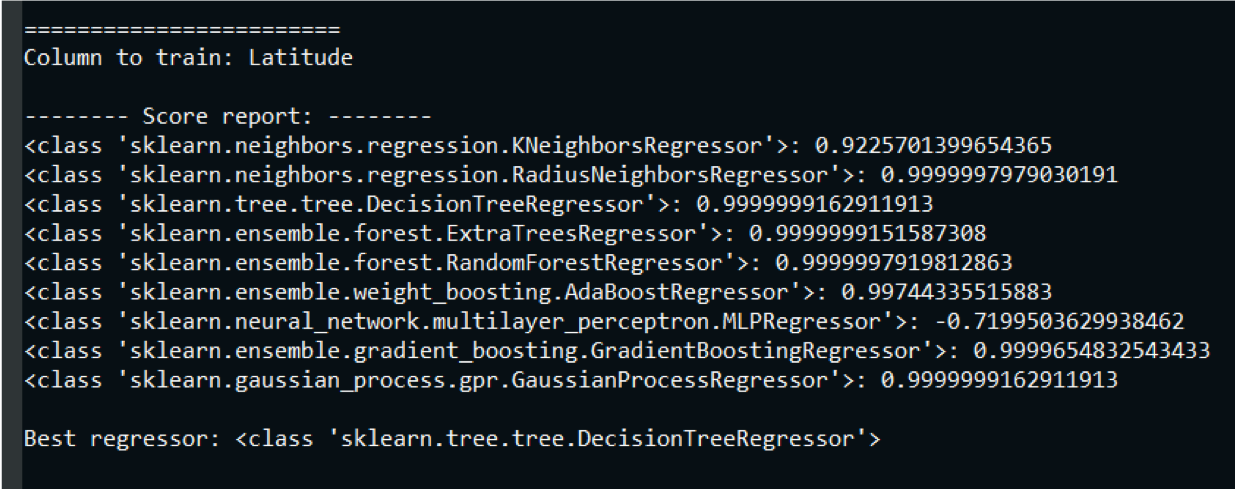
\includegraphics[width=\columnwidth]{img/output-accuracy.png}}
\caption{Example $R^2$ scores for a column inside the reference dataset for various regressors.}
\label{accuracy}
\end{figure}

SheetComplete was designed to be extensible and algorithm-agnostic; it doesn't use any algorithm-specific functionality. However, since it relies on the built-in \texttt{.score} property of the regressors, only regressors that have use the $R^2$ function to determine their score were enabled. Therefore, SheetComplete does not test the full suite of multi-output regressors in \texttt{scikit-learn}. 

\section{Conclusion \& Next Steps}
SheetComplete served as a very useful learning tool, as we were completely unfamiliar with machine learning concepts or implementations at the beginning of the project, and were entirely self-taught through the process. Although SheetComplete is incomplete (despite its name), we have identified concrete improvements that can be explored for future iterations of the application.

Future work may involve improving the scoring mechanism, which currently uses the $R^2$ score from its single test/train split. This may be improved by using \textit{cross-validation}: a process of testing the model's prediction accuracy with multiple test/train splits (i.e. averaging the prediction ability across subsets of the same larger dataset). The authors intuit that this improvement will have a more noticeable impact on smaller sheets, as data anomalies can more easily skew the regressors with smaller datasets.

Furthermore, SheetComplete can be extended to work on non-numerical datasets as well. Although we set out to include this functionality during the project's proposal phase, we were unable to implement it due to a lack of time and understanding of machine learning techniques. Some non-numerical data is easy to quantify (e.g. dates can be turned into days before/since some epoch), but others prove very challenging. With no theoretical background in machine learning, it is difficult to choose between categorization (e.g. one-hot encoding for each unique string), conversion (e.g. some numerical representation of each character), or some other technique unknown to us.

Other research may be able to influence future SheetComplete work as well. \cite{nural_using_2017} has identified that \textit{meta-learning} may be useful as a technique to better assess classifier/regressor performance in data analysis. Essentially, it uses characteristics of the dataset, features, algorithm selection, and algorithm performance to optimally select dataset--algorithm pairs. 

\balance

This strategy may also be able to fine-tune algorithm parameters to achieve better accuracy. For example, the \textit{k-nearest neighbours} algorithm (implemented in \texttt{KNeighborsRegressor}) will perform differently dependent on its value for $k$. If SheetComplete is run on a sufficient variety of test sheets, trends may emerge that match dataset types (e.g. dates, integers, latitude/longitude coordinates) or patterns (e.g. categorical, linear, random) to specific algorithms. In this case, SheetComplete's algorithm could be fine-tuned using these additional insights.

Research into spreadsheet property detection is also ongoing. \cite{chen_spreadsheet_2017} discusses a machine learning framework -- assisted by pre-defined rules -- to discover properties of individual data collections within a spreadsheet, and to extract unique datasets. Future iterations of SheetComplete may integrate this work to better extract uniform datasets from spreadsheets with complex layouts (e.g. headers, multiple data directionality, etc.). 

It is also possible to generalize SheetComplete to work in a more structured manner (i.e. without intuiting data set orientation and placement). In other words, SheetComplete may accept information about dimensions and locations of data sets from a user. For example, if SheetComplete was implemented as an add-on to Microsoft Excel (with a VBA wrapper), the function could receive the dimensions and location of a highlighted area within a sheet to more rigidly define the locations of datasets.

\section*{Source Code}
Source code for this project is freely available at \mbox{\url{https://github.com/squircle/sheetcomplete}}. SheetComplete is freely licensed under the GNU General Public License version 3 (GPL-3.0).

\bibliography{sheetcomplete.bib}

\end{document}
